\documentclass[12pt]{article}

\usepackage{t1enc}
\usepackage[utf8]{inputenc}
\usepackage[magyar]{babel}
\usepackage{amsmath}
\usepackage{amsfonts}
\usepackage{amsthm}
\usepackage{amssymb}
\usepackage{enumerate}
\usepackage[shortlabels]{enumitem}
\usepackage[autostyle]{csquotes}
\usepackage{graphicx}


\selectlanguage{magyar}

\DeclareQuoteAlias{dutch}{magyar}

\theoremstyle{definition}
\newtheorem{definition}{Definíció}
\newtheorem*{definition*}{Definíció}

\let\oldemptyset\emptyset
\let\emptyset\varnothing

\newcommand{\forwardhat}{\overset{\rightharpoonup}}
\newcommand{\backwardhat}{\overset{\leftharpoonup}}

\newcommand{\inc}{\textit{inc}}
\newcommand{\dec}{\textit{dec}}

\graphicspath{ {./images/} }


\title{Reverzibilis Reaction System}
\date{\today}

\begin{document}
    \maketitle

    \begin{definition*}
        Az $\mathcal{A} = (S, A)$ \textit{reaction system} reverzibilissé tehető, amennyiben teljesülnek a következő feltételek:
        \begin{enumerate}[label={(\arabic*)}]
            \item
            $\mathcal{A}$ nem tartalmaz olyan reakciókat, melyeknek jobb oldala átfedő: tetszőleges $i, j \in A$ reakció esetén $P_{i} \cap P{j} = \emptyset$, ha $i \neq j$.

            \item
            A kontextusból kapott szimbólumok nem állhatnak elő egy reakció produktumaként sem: ha $\pi = (\gamma, \delta)$ egy \textit{interactive process}, ahol $\gamma = C_{0}, C_{1}, \ldots, C_{n}$, $n \geq 1$, akkor bármely $C_{i}$ kontextus és $a \in A$ reakció esetén $C_{i} \cap P_{a} = \emptyset$.

            \item
            Az állapotok minden eleme részt vesz valamilyen reakcióban: ha $\pi$ egy \textit{interactive process}, ahol $\textit{sts}(\pi) = W_{0}, W_{1}, \ldots, W_{n}$, $n \geq 1$, akkor $\bigcup_{a \in \textit{en}(W_{i})} R_{a} = W_{i}$, $i \leq n$.
        \end{enumerate}
        Ekkor az $\mathcal{A}$-nak megfelelő reverzibilis \textit{reaction system} $\mathcal{A}_{\textit{rev}} = (S_{\textit{rev}}, A_{\textit{rev}})$, ahol
        \begin{align*}
            S_{\textit{rev}} &= S \cup \{ \, \rho \, \}, \\
            A_{\textit{rev}} &= \forwardhat A \cup \backwardhat A, \\ 
            \forwardhat A &= \{ \, (R_{a}, I_{a} \cup \{ \, \rho \, \}, P_{a}) \; : \; a \in A \, \}, \\
            \backwardhat A &= \{ \, (P_{a} \cup \{ \, \rho \, \}, \emptyset, R_{a}) \; : \; a \in A \, \}.
        \end{align*}
        $\rho$ egy speciális szimbólum (tehát $\rho \notin P_{a}, a \in A_{\textit{rev}}$), mely egy visszafelé irányba tett számítási lépésre kényszeríti a rendszert.
    \end{definition*}

    \section*{Példa}
    Tekintsünk a \textit{Tour of Reaction Systems} cikkből egy olyan \textit{Binary Countert}, ahol $n = 2$, azaz két bittel dolgozunk. Ekkor a \textit{reaction system} a következő alaphalmazból és reakciókból áll:

    \begin{align*}
        S = \; & \{ \, p_{0}, p_{1},  \inc, \dec \, \}, \\
        A = \; & \{ \\
            & \quad (\{ p_{0} \}, \{ \dec, \inc \}, \{ p_{0} \}), \\
            & \quad (\{ p_{1} \}, \{ \dec, \inc \}, \{ p_{1} \}), \\
            & \quad (\{ \inc \}, \{ \dec, p_{0} \}, \{ p_{0} \}), \\
            & \quad (\{ \inc, p_{0} \}, \{ \dec, p_{1} \}, \{ p_{1} \}), \\
            & \quad (\{ \inc, p_{1} \}, \{ \dec, p_{0} \}, \{ p_{1} \}), \\
            & \quad (\{ \dec \}, \{ \inc, p_{0}, p_{1} \}, \{ p_{1} \}), \\
            & \quad (\{ \dec \}, \{ \inc, p_{0} \}, \{ p_{0} \}), \\
            & \quad (\{ \dec, p_{0}, p_{1} \}, \{ \inc \}, \{ p_{1} \}), \\
        \; &\}
    \end{align*}

    Az így kapott \textit{rs} nem teljesíti a fenti definíciót, hiszen a reakciók jobb oldalai között lesz átfedés. Ezt jobban illusztrálja, ha állapotátmenet-diagramon ábrázoljuk a rendszer működését (egyelőre kihagyva a \textit{reset} átmenetet, amikor a bemenet az $\inc$ és $\dec$ szimbólumokból áll):

    \begin{figure}[h]
        \centering
        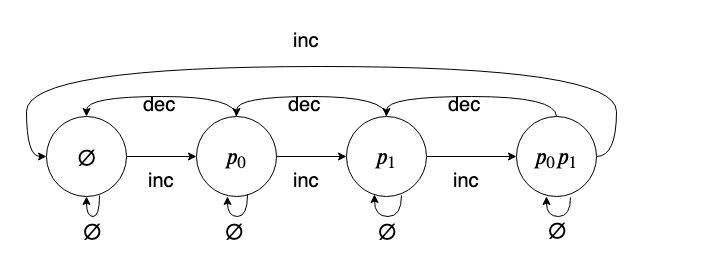
\includegraphics[width=5in]{two-bit-counter-states.jpg}
    \end{figure}

    Ha például a $p_{0}$ állapotban vagyunk, akkor nem tudhatjuk, hogy az üres állapotból, önmagunkból vagy a $p_{1}$ állapotból érkeztünk, azaz, a megelőző lépés növelés, helyben maradás vagy csökkentés volt-e. Így a visszalépés nem egyértelmű.

    Kettőnél több bit esetén a definíció harmadik szabálya sem teljesül, hiszen ahogy a cikkben szerepel, lehetnek eltűnő szimbólumok (\enquote{\textit{[When an increment is requested] bits that are less significant than the $2^{j}$ position will disappear because there are no enabled reactions to produce them.}}).
\end{document}
